\subsubsection{\stid{5.06} Flang}\label{subsubsect:flang}

\paragraph{Overview}
The Flang project provides an open source Fortran
\cite{iso-fortran-2004} \cite{iso-fortran-2010} \cite{iso-fortran-2018}
compiler licensed and designed
for integration with the LLVM Compiler Infrastructure (see \url{http://llvm.org})~\cite{llvm:homepage}.
The Flang compiler is a cross-platform Fortran solution for multicore CPUs available
to ECP and HPC users today. Goals of the project include extending support to GPU
accelerators and Exascale systems, and supporting LLVM-based software and tools
R\&D of interest to a large deployed base of Fortran applications.  With the growing
popularity and wide adoption of LLVM within the broader HPC community, this project
provides the foundation for a Fortran solution that will complement and interoperate
with the Clang/LLVM C++ compiler.  It will allow Fortran to grow into a modernized
open source form that is stable and has an active footprint within the LLVM
community, and will meet the needs of a broad scientific computing community.  The
Flang source code base is derived from the well-established PGI/NVIDIA proprietary
Fortran compiler, which provides a solid compiler base from which to evolve a
Fortran front-end and runtime libraries coded in a style which will allow new
contributors to ramp up and be productive quickly.  The most active developers
continue to be PGI/NVIDIA, with recent contributions from ARM Ltd and the DOE
National Labs demonstrating a path to long-term sustainability.  Full source is
available at \url{https://github.com/flang-compiler/flang}, and mailing lists and a
Slack channel have been created (\url{http://lists.flang-compiler.org/} and
\url{http://flang-compiler.slack.com/} respectively).

\paragraph{Key Challenges}
There are several commercially-supported Fortran compilers, typically available on
only one or a few platforms.  None of these are open source.  The GNU gfortran
open source compiler is available on a wide variety of platforms, but the source
base is not modern LLVM-style C++, and the GPL open source license is not compatible
with LLVM. As a result, leveraging gfortran in the LLVM community is problematic.
The primary challenge of this project is to create a source base with the maturity,
features and performance of proprietary solutions, the cross-platform capability
of GNU compilers, and which is licensed and coded in a style that will be embraced
by the LLVM community.  Another key challenge is robustly supporting all Fortran
language features, programming models and scalability that will be required for
effective use on Exascale systems, and balancing project resources across immediate
bug fixes and minor requests-for-enhancement versus the strategic requirement to
modernize the source code base.

\paragraph{Solution Strategy}
The Flang project strategy was and is to streamline (remove unused legacy code,
modify source to compile cleanly with no Clang warnings, minimize or eliminate use
of conditional compilation, incremental migration to C++) and integrate the
existing PGI Fortran front-end with LLVM's opt/llc components to create an open
source baseline compiler with the same Fortran language and OpenMP features as
the commercial PGI Fortran compiler.  From that baseline compiler, additional
Fortran language and OpenMP features will be added while tracking the evolution
of LLVM closely from release-to-release.  Also from that baseline compiler, selected
components will be prioritized for significant refactoring or re-writing as required
to meet the requirements of the LLVM community, to enable LLVM developers to
easily ramp up and contribute, and to support all of modern Fortran and its
related programming models in a fully robust way across all supported platforms.

The above significant refactoring of Flang is embodied in the subproject we call
\emph{F18}, which is a new C++ Fortran front-end aligned with modern software
principles and LLVM coding standards. The goal is for F18 to be adopted as a
full LLVM project, and that for F18 to replace the current Flang front-end when
its support of Fortran standards and HPC programming models exceeds current Flang's.

\paragraph{Recent Progress}
Recent developments have added support for additional Fortran debugging metadata
(including effort to upstream LLVM changes into their code base),
initial support for GPU offload for OpenMP 4.5 \cite{openmp-spec-45} based on
Clang's support for GPU offload,
support for Fortran 2018 DO CONCURRENT and
Fortran 2008 SUBMODULE and internal procedure pointers,
and improvements to the \emph{libpgmath} infrastructure for optimized
scalar and SIMD Fortran numerical intrinsics. With these in place, Flang delivers
performance averaging 5\% faster than gfortran across a range of benchmarks and
enables ECP developers to write and test OpenMP 4.5 on multicore CPU targets.

We continued development on the F18 Fortran 2018 parser and released this to the
Flang community on GitHub.
F18 is able to parse full the full Fortran 2018 language,
and perform semantic analysis on symbols, expressions,
types, modules and submodules.
We are designing the control flow graph structure and beginning
to support translation of the Fortran ASTs to the CFG.

\

Figure~\ref{fig:flang-performance} illustrates the relative performance of Flang against gfortran.

\begin{figure}[htb]
	\centering
	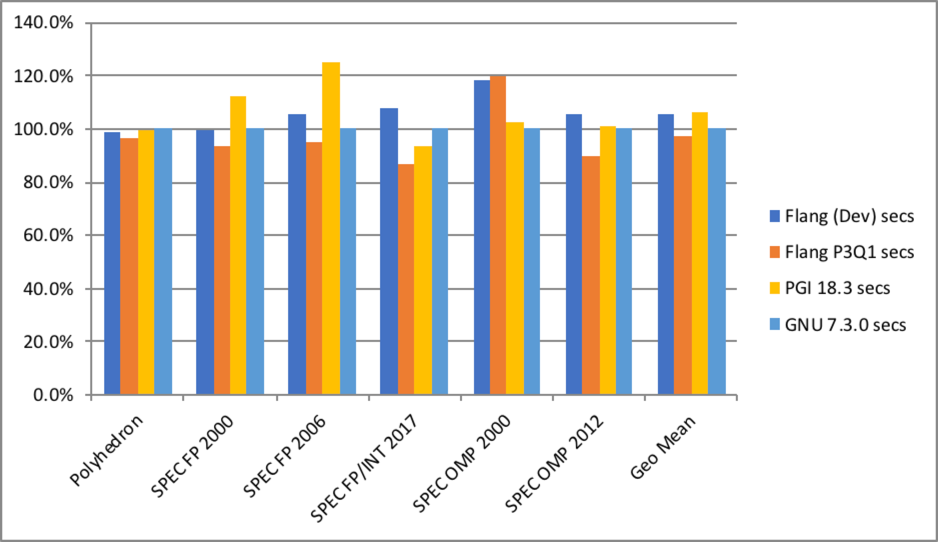
\includegraphics[width=6in]{projects/2.3.5-Ecosystem/2.3.5.06-Flang/flang-performance}
	\caption{\label{fig:flang-performance}Flang performance is benchmarked against other Fortran compilers. The above diagram shows the relative performance of Flang against PGI Fortran and GNU gfortran}
\end{figure}

\paragraph{Next Steps}
We have recently added work on OpenMP 4.5 target offload support for NVIDIA Tesla
GPUs to Flang open source.
We will continue work on robustness of the GPU targeting for the remainder of 2019.

As we work through these aspects of modernization, we will continue to build up the Flang
testing infrastructure and be as responsive as possible to bug reports and minor
requests for enhancement from what will hopefully be a growing base of Flang users
in the ECP and HPC communities.

We will continue development on the F18 Fortran 2018 parser, increasing our resource
investment and outreach to other compiler development teams associated with ECP.
We will complete design of the control flow graph (CFG) structure
and will continue to work on translation of the Fortran ASTs to the CFG.
We will work to get early feedback on the structure of F18 for the development
of Fortran-specific programming tools.

We plan to achieve formal adoption of F18 as an LLVM subproject in 2019.
